% Requires:
% \usepackage{amsmath}
% \usetikzlibrary{angles}
% \usetikzlibrary{calc}
% \usetikzlibrary{fit}
% \providecommand{\bsit}[1]{\boldsymbol{#1}}
% INCLUDE ../images/random-scene.png relto ../main.tex
\begin{tikzpicture}[
    scale=0.75,
    every node/.style={transform shape},
  ]
  \makeatletter
  \tikzset{
    fitting node/.style={
      inner sep=0pt,
      fill=none,
      draw=none,
      reset transform,
      fit={(\pgf@pathminx,\pgf@pathminy) (\pgf@pathmaxx,\pgf@pathmaxy)}
    },
    reset transform/.code={\pgftransformreset}
  }
  \makeatother

  \pgfdeclarelayer{background}
  \pgfsetlayers{background,main}
  \node[rounded corners,thick,draw,align=center] (rsg) {Random scene\\generator};
  \node[rounded corners,thick,draw,align=center,below of=rsg,node distance=1.2cm] (buffer) {Replay\\buffer};

  \path (rsg.east) -- ++(1.,0) node[circle,draw,fill,inner sep=1.5pt] (out_rsg) {};
  \path (buffer.east) -- (out_rsg |- buffer.east) node[circle,draw,inner sep=1.5pt] (out_buffer) {};
  \draw[thick] (rsg) -- (out_rsg);
  \draw[thick] (buffer) -- (out_buffer) node[midway,above,font=\footnotesize] {scene};

  \path ($(out_rsg)!0.5!(out_buffer)$) -- ++(1,0) node[circle,draw,fill,inner sep=1.5pt] (choose_scene) {};
  \draw[thick] (choose_scene) -- ++(.5,0) node[right] (input_scene) {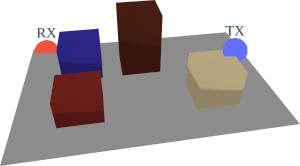
\includegraphics[width=2cm]{images/random-scene.png}};
  \draw[thick] (choose_scene) -- (out_rsg) node[above,midway,sloped,font=\footnotesize] {$u_\text{s} > \alpha$};
  \draw[thick,dashed] (choose_scene) -- (out_buffer) node[below,midway,sloped,font=\footnotesize] {$u_\text{s} \leq \alpha$};
  \pic[draw,dashed,<->,angle radius=.6cm,angle eccentricity=1,font=\footnotesize,pic text={$u_\text{s}\sim\mathcal{U}(0,1)$},anchor=east] {angle = out_rsg--choose_scene--out_buffer};

  \path (input_scene.east) -- ++(1.5,0) node[anchor=west,align=center] (sampler_txt) {Generative\\Path Sampler};

  \path (sampler_txt.north) -- ++(.7,1) node[circle,draw,fill,inner sep=1.5pt] (choose_policy) {};

  \begin{scope}[local bounding box=sampling_policy]
    \draw[thick] (choose_policy) -- ++(-1,.5) node[midway,above,sloped,font=\footnotesize] {$u_\pi>\epsilon$} node[circle,draw,fill,inner sep=1.5pt] (flow_policy) {} -- ++(-.5,0) node[left] (policy) {$\pi_{\bsit{\theta}^{(i)}}$};
    \path (choose_policy) -- ++(-1,-.5) node[circle,draw,inner sep=1.5pt] (uniform_policy) {};
    \draw[thick,dashed] (choose_policy) -- (uniform_policy) node[midway,below,sloped,font=\footnotesize] {$u_\pi\leq\epsilon$};
    \draw[thick] (uniform_policy) -- ++(-.5,0) node[left] (policy) {$\pi_{\mathcal{U}}$};
    \pic[draw,dashed,<->,angle radius=.6cm,angle eccentricity=1,font=\footnotesize,pic text={$u_\pi\sim\mathcal{U}(0,1)$},anchor=east] {angle = flow_policy--choose_policy--uniform_policy};
    \draw[thick] (choose_policy) -- ++(.5,0) node[right] {$\pi$};
  \end{scope}
  \begin{pgfonlayer}{background}
    \node[draw=blue,thick,rounded corners,fill=blue!20,fit={(sampler_txt) (sampling_policy)}] (sampler) {};
    \filldraw[thick,dashed,rounded corners,draw,fill=blue!05] (sampling_policy.north west) rectangle (sampling_policy.south east);
  \end{pgfonlayer}
  \draw[->,thick] (input_scene.east) -- (sampler.west |- sampler_txt.west);
  \draw[->,thick] (sampler.east) -- ++(.5,0) node[anchor=west,rounded corners,thick,draw,align=center,draw,fill=gray!20] (pt) {Path\\Tracing};
  \draw[->,thick] (pt.east) -- ++(.5,0) node[anchor=west,rounded corners,thick,draw,align=center,draw,fill=gray!20,label={[font=\footnotesize,align=center]below:{Computes\\reward ($r$)}}] (gv) {Geometric\\Validation};

  \draw[<-,thick,dashed,rounded corners] ([yshift=+0.3cm]sampler.south west) -- ++(-.5,-.6) -- ([yshift=-0.3cm]buffer.east) node[midway,below,font=\footnotesize] {Path candidate (only used during replay)};

  \draw[->,thick] (sampler.north) -- ++(0,.5) node[midway,left,font=\footnotesize] (flows) {$\bsit{F}_{\bsit{\theta}^{(i)}}$} node[above,thick,draw,rounded corners] (loss_grads) {$\nabla_{\bsit{\theta}} \mathcal{L}$};
  \draw[->,thick,rounded corners] ($(sampler.east)!0.3!(pt.west)$) |- ([yshift=-0.1cm]loss_grads.east) coordinate[pos=0] (x_pc);
  \draw[->,thick,rounded corners] (gv.east) -- ++(0.3cm,0) |- ([yshift=0.1cm]loss_grads.east);

  \draw[<-,thick] (sampler.west |- sampling_policy.west) -- ++(-0.7,0) node[anchor=east,label={[align=center,above=.8em,font=\footnotesize]Current model\\parameters}] (params) {$\bsit{\theta}^{(i)}$};

  \draw[<-,thick] (params.west) -- ++(-2.5,0) node[anchor=east,draw,rounded corners,label={[align=center,name=optims_label,above=.8em,font=\footnotesize]Update model\\parameters}] (optims) {Optimizer} node[midway,above,font=\footnotesize] {$\bsit{\theta}^{(i+1)}\rightarrow\bsit{\theta}^{(i)}$};
  \draw[->,thick,rounded corners] (params.south) -- ++(0,-.3cm) -| (optims.south);
  \draw[<-,thick] (optims.west) -- ++(-0.8,0) node[circle,draw,anchor=east,inner sep=1pt] (acc) {$\bsit{+}$};
  \node[font=\footnotesize,align=center,anchor=north] at (acc.north |- optims_label.north) {Accumulate\\batches};

  \path (x_pc) -- ([yshift=-.5cm]x_pc |- buffer.south) coordinate (tmpA) -- (buffer.south |- tmpA) coordinate[pos=.85] (tmpB);
  \path (tmpA) -- (tmpB) node[midway,below,font=\footnotesize] {Insert new path candidate (not from replay buffer)};

  \draw[thick,rounded corners] (x_pc) |- (tmpB) node[circle,draw,fill,inner sep=1.5pt] (tmpC) {};
  \path (tmpC) -- ++(225:.6cm) node[circle,fill,draw,inner sep=1.5pt] (tmpD) {};
  \path (tmpC) -- ++(180:.6cm) node[circle,draw,inner sep=1.5pt] (tmpE) {};
  \path (tmpC) -- ++(270:.4cm) coordinate (arc_start);
  \draw[thick] (tmpC) -- (tmpD);
  \draw[->,thick,rounded corners] (tmpE) -| (buffer.south);
  \draw[->] (arc_start) arc (270:180:.4cm);

  \node[anchor=north west,font=\footnotesize] (if_success) at (arc_start) {if $r>0$};
  \draw[->,thick,rounded corners] (gv.east) -- ++(.3cm,0) |- (if_success.east);

  \draw[->,thick,rounded corners] (loss_grads.west) -| (rsg.west |- params) -- (acc.west);

\end{tikzpicture}
